\chapter{Requirement Analysis}

\subsection{Relevant Human and Non-Human Actors}

\textbf{Human Actors:}
\begin{itemize}
    \item \textbf{Traffic Managers} – Access daily reports (Type 1), review and approve/reject optimization proposals (Type 2 and Type 3).
    \item \textbf{Citizens} – Receive real-time traffic data (Type 1), and event-based routing suggestions (Type 2, 3) through the application.
    
    \item \textbf{Event Organizers} – Submit data about upcoming public events (Type 3).
\end{itemize}



\textbf{Non-Human Actors:}
\begin{itemize}
    \item \textbf{Sensor System} – Event-based system that provides real-time traffic flow data (Type 1).
    \item \textbf{Public Transport Microservice} – Provides public transportation timetables (Type 2, Type 3).
    \item \textbf{Public Transport Schedulers} – Provide bus/tram schedules in response to accepted system recommendations (Type 2 and 3).
    \item \textbf{Traffic Light System} – Accepts dynamic configuration changes (Type 1 and 3).
    \item \textbf{News Channel} – Publishes upcoming events (Type 3).
    
\end{itemize}

\newpage
\subsection{Use Cases}

This section describes the main use cases of the UrbanLeaf System. The use cases model the interactions between external actors (citizens, managers, event organizers, sensors, and other systems) and the functionalities provided by the application. These interactions are visualized in the use case diagram below.

\vspace{1em}
\begin{center}
    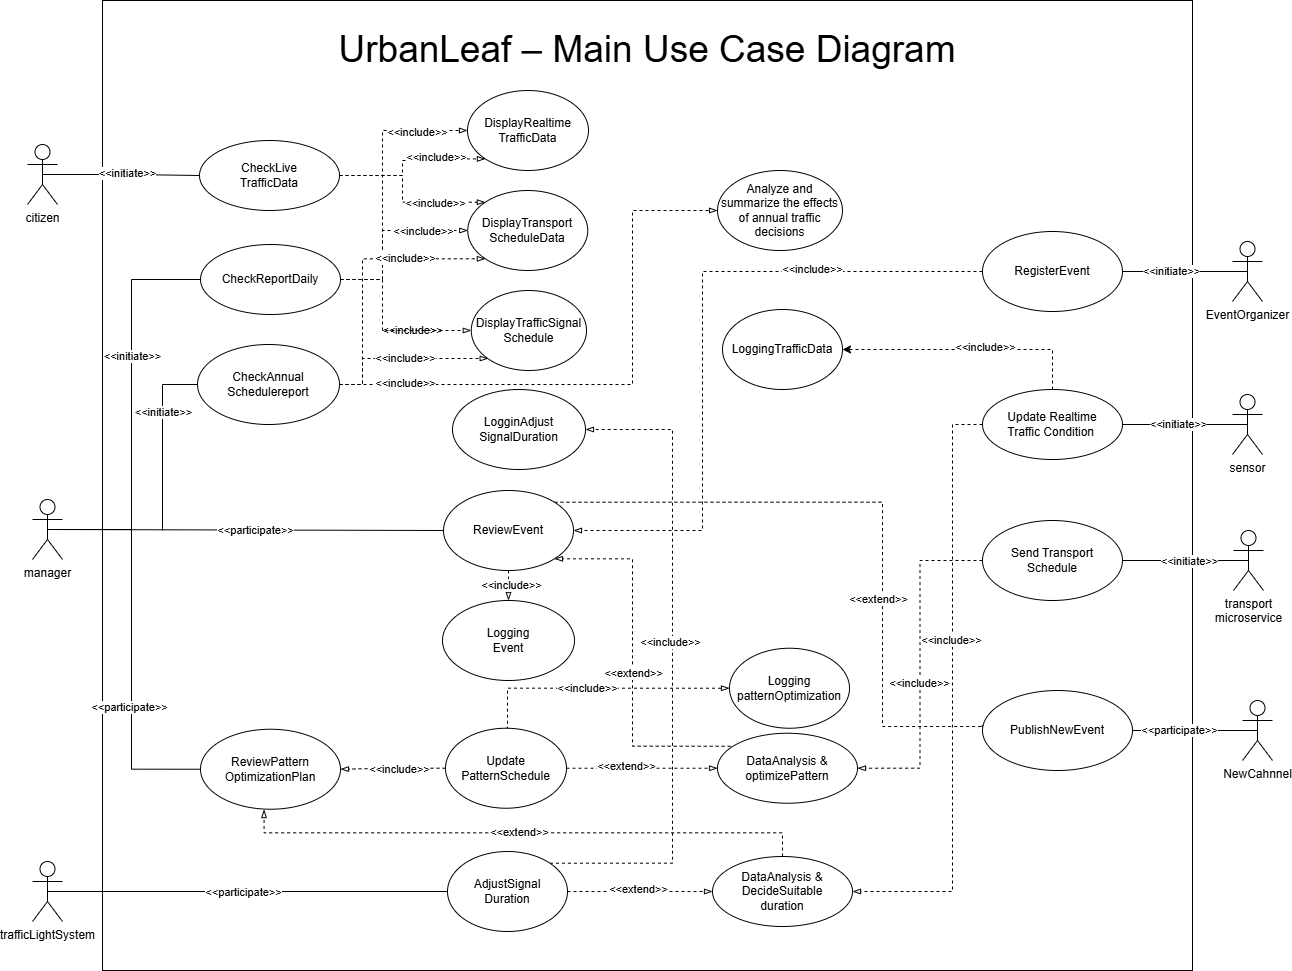
\includegraphics[width=1\textwidth]{Images/UseCase.png}
\end{center}
\vspace{1em}

\subsubsection*{Overview of Represented Use Cases}

\begin{itemize}
    \item \textbf{CheckLiveTrafficData}: Citizens access real-time traffic information through the app. This use case includes:
    \begin{itemize}
        \item \textit{DisplayRealtimeTrafficData}
        \item \textit{DisplayTransportScheduleData}
        \item \textit{DisplayTrafficSignalSchedule}
    \end{itemize}

    \item \textbf{CheckReportDaily / CheckAnnualScheduleReport}: Managers view daily and yearly traffic-related reports. The annual report includes system decisions and long-term insights.

    \item \textbf{RegisterEvent}: Event organizers register upcoming public events, including location, time, and estimated attendance.

    \item \textbf{UpdateRealtimeTrafficCondition}: The sensor system sends continuous real-time traffic flow data to the application.

    \item \textbf{SendTransportSchedule}: The public transport microservice provides schedules for buses and trams, which are used by the system to plan responses.

    \item \textbf{ReviewEvent / ReviewPatternOptimizationPlan}: Traffic managers access the dashboard to review system-generated suggestions related to events or recurring traffic patterns.

    \item \textbf{UpdatePatternSchedule / AdjustSignalDuration}: Once suggestions are approved by managers, the system updates transport schedules or modifies signal timing accordingly.

    \item \textbf{PublishNewEvent}: The News Channel actor receives and publishes relevant traffic and event information for public visibility.

    \item \textbf{LoggingTrafficData, LoggingEvent, LoggingPatternOptimization}: All key actions are recorded for traceability, report generation, and audit purposes.
\end{itemize}

\subsubsection*{Additional Use Cases (Not Represented in Diagram)}

In addition to the diagrammed use cases, the following functionalities are part of the system's behavior:

\begin{itemize}
    \item \textbf{Notify Rerouting Information to Citizens (T1, T3)}: Citizens receive personalized routing suggestions in case of detected congestion or planned events.

    \item \textbf{Handle System Errors and Log Failures (All)}: The system monitors component interactions and logs any data or service-related failures.

    \item \textbf{Generate Optimization Suggestions (T2)}: The pattern analyzer periodically identifies trends and proposes transport or traffic optimizations.

    \item \textbf{Analyze Event Impact (T3)}: The event analyzer estimates the traffic impact of upcoming public events using both live and historical data.

    \item \textbf{Summarize Traffic and System Performance (T1, T2, T3)}: Periodic and event-triggered summaries are generated for use in daily and annual reports.
\end{itemize}

Together, these use cases represent the functional core of the system and form the basis for the requirements described in the following section.



\newpage
\subsection{Domain Assumptions}
\begin{itemize}

  \item \textbf{Traffic Infrastructure}
  \begin{itemize}
    \item Traffic sensors are installed throughout the city and continuously provide real-time data.
    \item Traffic lights can be adjusted by the system in real time.
    \item A public transport infrastructure exists with modifiable and plannable schedules.
    \item Historical traffic and transport data are available for pattern analysis.
  \end{itemize}

  \item \textbf{Actors and Stakeholders}
  \begin{itemize}
    \item Managers are authorized to approve or reject proposed traffic and transport changes.
    \item Citizens use a mobile or web-based application to access real-time traffic updates.
    \item Event Organizers can submit structured event information.
    \item All actors interact with the system through predefined interfaces or components.
  \end{itemize}

  \item \textbf{Communication and Data Handling}
  \begin{itemize}
    \item Real-time and scheduled data flows through the Data Aggregator to other modules.
    \item The system’s App is capable of pushing notifications and updates to citizens.
    \item The Logger module is always available to record actions, suggestions, and system responses.

  \end{itemize}

  \item \textbf{System Capabilities}
  \begin{itemize}
    \item The pattern analyzer can identify optimizations based on both historical and real-time data.
    \item The analyzers are capable of generating temporary or permanent changes to schedules or signals.
    \item Suggested optimizations may include schedule adjustments, signal duration, or rerouting.
  \end{itemize}
\end{itemize}



\newpage
\subsection{Requirements}
\subsubsection{Functional Requirements}

\begin{itemize}
    % Task 1
    \item FR1.1: Receive real-time traffic data from sensors every 30 seconds.
    \item FR1.2: Detect road congestion and dynamically adjust light durations.
    \item FR1.3: Log all light adjustments with time, location, and change details.
    \item FR1.4: Generate and publish daily reports to authorized managers via the application.
    \item FR1.5: Display real-time traffic updates to citizens via application.

    % Task 2
    \item FR2.1: Analyze historical traffic patterns over days.
    \item FR2.2: Suggest light timing changes for high-traffic zones.
    \item FR2.3: Recommend public transport schedule changes based on congestion patterns.
    \item FR2.4: Present all suggestions to traffic managers and log their decisions.
    \item FR2.5: Generate yearly reports listing all Type 2 suggestions with status.

    % Task 3
    \item FR3.1: Collect upcoming event data from Public Transport Microservice, Data Aggregator and event organizers.
    \item FR3.2: Assess traffic impact using historical and live data.
    \item FR3.3: Suggest temporary traffic configurations and transport updates.
    \item FR3.4: Notify users with personalized routing and event alerts.
    \item FR3.5: Generate yearly reports of Type 3 suggestions and approvals.
\end{itemize}


\newpage
\subsubsection{Non-Functional Requirements}
\begin{itemize}
    \item \textbf{NFR1.1}: The system shall respond to real-time sensor data updates with low latency under typical traffic conditions (Type 1).
    \item \textbf{NFR1.2}: Historical data analyses shall complete in a timely manner to support periodic reviews and long-term planning (Type 2).
    \item \textbf{NFR1.3}: Event-based suggestions shall be generated promptly upon data reception to enable early planning and action (Type 3).
    \item \textbf{NFR1.4}: All logged actions and decisions shall be securely stored, timestamped, and protected from tampering.
    \item \textbf{NFR1.5}: Reports shall be available in a standardized digital format suitable for archival and sharing (e.g. PDF).
    \item \textbf{NFR1.6}: The system interfaces shall be accessible, user-friendly, and optimized for use on both desktop and mobile devices.
    \item \textbf{NFR1.7}: Access to administrative and decision-making features shall be controlled through role-based permissions.
    \item \textbf{NFR1.8}: The system shall scale to support multiple simultaneous analyses and event-handling processes without loss of functionality.
    \item \textbf{NFR1.9}: Communication between system components shall be efficient and consistent to avoid bottlenecks and delays.
    \item \textbf{NFR1.10}: The system shall maintain data integrity when handling concurrent operations such as logging and configuration updates.
    \item \textbf{NFR1.11}: During periods of high activity, critical event-handling operations shall be prioritized over routine background tasks.
\end{itemize}